\documentclass[11pt,a4paper,portrait]{article}

\usepackage{polytechnique}
\usepackage[utf8x]{inputenc}
\usepackage[T1]{fontenc}
\usepackage[english]{babel}

\usepackage{amsmath}
\usepackage{amsfonts}
\usepackage{amssymb}
\usepackage{amsthm}
\usepackage{graphicx}
\usepackage{hyperref}
\usepackage{polytechnique}


\author{Nicolas Drizard, Eloi Zablocki, INF582$\_$42}
\date{March, 1st 2015}
\title{Predicting Survival on the Titanic Wreck}


\begin{document}

\maketitle


\newpage
\part*{Introduction}
In the report we present our approach to the \textit{Kaggle} competition\footnote{More info to be found at \url{https://www.kaggle.com/c/titanic-gettingStarted/}}. The goal is to predict the passengers that survived at the shipwreck of Titanic, given some caracteristics such as the genre, the age, etc.\\
First, we will explain the preprocessing task that has been made in order to clean, extract and create features. Then we will go through the classification task, with the algorithms used and tried.

\part{\textit{Data pre-processing} and \textit{Feature Engineering}}
\setcounter{section}{0}


\section{Data pre-processing}
As given with the assignment, the data of \textit{train.csv} and \textit{test.csv} were composed of raws and there was some work to be done in order to clean the data. For example, there are missing values in the dataset, some features are not useful such as the passengerId, some features are string with very useful information such as the passenger name (containing the title and the family name).

\paragraph{Use of pandas}
To easily clean up the data set and create new features, we have used the python library \textit{pandas}. This library allowed to visualize and explore data.

\paragraph{Data visualization}
One of the first tasks we made was data visualization. Indeed, in order to have some insights on the general pipeline, it is very convenient to visualize the data. For example, our first observation was the part of women who have survived compared to the part of the men who have survived. Here you can find some visualizations (Figure~\ref{sexsur}, Figure~\ref{agesur}, Figure~\ref{titlesur}) made on Weka (the software used will be presented later in this report). The color blue represents the people who died and the red color the survivors.

\begin{figure}[!ht]
	\centering
	\begin{minipage}[t]{5.5cm}
		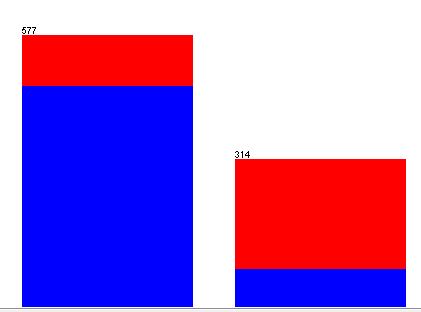
\includegraphics[scale=0.6]{sexsur.png}
		\caption{Dead and surviving people repartition functions of the sex. Left : Male, Right : Female}
		\label{sexsur}
	\end{minipage}
	\begin{minipage}[t]{5.5cm}
		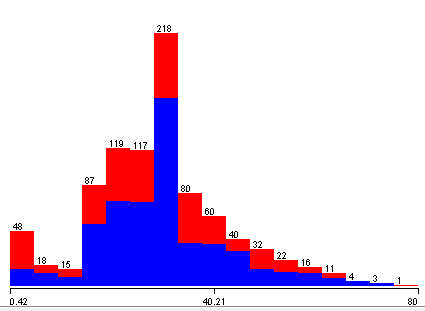
\includegraphics[scale=0.6]{agesur.png}
		\caption{Dead and surviving people repartition functions of the age}
		\label{agesur}
	\end{minipage}
	\begin{minipage}[t]{5.5cm}
		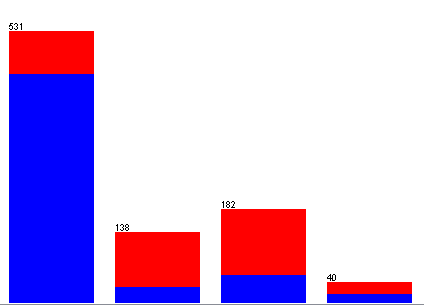
\includegraphics[scale=0.6]{titlesur.png}
		\caption{Dead and surviving people repartition functions of the title.
	From the left to the right : Mr, Mrs, Miss, Master}
		\label{titlesur}
	\end{minipage}	
\end{figure}



\section{Feature Engineering}

\subsection{Creation of features}

\paragraph{Feature extraction}
Some features such as the name and the cabin number contain precious information such as the title or the deck number. Nevertheless most of the algorithms would have troubles to use those features since they are strings. Thus, a "hand-made" extraction of the features has to be done.

\subparagraph{Title extraction}
The title can give useful information on a person. A Lord, a Master (children), and a Miss have all three different chances to survive. With some appropriate function of \textit{pandas} we have extracted the title from the name of the person. This gives us about 15 titles in the training set. We have aggregated the titles into four representative categories so that our algorithm is less likely to overfit the data. The categories are Mr., Miss., Mrs. and Master. To sum up, we have created a four-categories feature "Title" and removed the feature "Name"


\subparagraph{Deck extraction}
Even though there are many missing values for the cabin number, those present give an information on which deck the person was. For example "C123" means that the cabin was on the deck "C". Again we have created a categorical feature "Deck" (values A, B, C, D, E, F, T, G or missing value) and removed the feature "Cabin".

\paragraph{New features}
Because we can always add or multiply two numbers to create a new number, here are the features that we have added to our dataset. Those features depends and are somehow redondant with other features.

\subparagraph{Family size}
We have created a "Family size" feature. This is simply equal to the sum of "Sibsp" (number or siblings and spouse) and "Parch" (number of parents and children) and it represents the size of the family.

\subparagraph{Fare per person}
We have created a "Fare per person" feature that is equal to the quotient of the "Fare" by the "Family size". The goal of this feature is to emphasize the difference between a single rich person and a poor person in a large family.

\subparagraph{Age class interaction}
We have created a "Age*class" feature. This feature is simply the product of the age of the person with his class. The goal of this feature is complementary to the "Fare per person" feature: it emphasizes the difference between an old rich man and a young poor person.


\subsection{Filling missing values}
Most of the algorithm implemented in Weka accept missing values. Thus we have only filled the missing values that are really important. Given that the age of the passenger is very important and that we do not want weka to replace the age of children with the average age of all the passengers, we have computed an approached age which is the mean of the age of people who have the same title. For example the average age of the Master children is 4.57 whereas the average age of Reverend people is 43.17.\\
This modification was extremely helpful to improve our score.


\part{Classification}
\setcounter{section}{0}

\section{Weka}
We chose to use an already built library to classify our cleaned data. Weka is a library developed by the Machine Learning group form the Waikato University\footnote{More info to be found at \url{http://www.cs.waikato.ac.nz/ml/}} in the Java programming language. Weka is a powerful tool for data analysis such as classification, regression, data vizualization or dimensionality reduction. In each of these machine learning fields, it has many implemented algorithms (50+ classification algorithms for example). Weka's input are \textbf{.arff} files which are very close to \textbf{.csv} files but with more information on the features.\\
The whole library accepts missing values and different kind of features (categorical, numerical, date...) yet some implemented algorithms may be more restrictive concerning the data type (some do not treat categorical features for example).\\
The preprocessing tasks explained in the part 1, gave us \textbf{.csv} files that we converted into \textbf{.arff} files, by hand. When Weka makes predictions on the test set, it returns an \textbf{.arff} file that we convert into \textbf{.csv} files, the accepted format for the \textit{Kaggle} submissions.

\section{Classification algorithm : REPTree}
The advantage of using the library Weka is that we can test our data set with many different algorithms. We have tried many algorithms such as Random Forest, AdaBoost, DecisionTable and so on. First note that the basic algorithm oneR that only takes into account the most important feature (sex) has a score of 0.765 on Kaggle.  An algorithm that does very well on our data and the features we have created is REPTree.\\
REPTree algorithm is a fast decision tree learner. It builds a decision tree using information gain and prunes it using reduced-erro pruning (with backfitting). In this algorithm, missing values are dealt with by splitting the corresponding instances into pieces. You can find the paper that describes the algorithm at \url{http://ictactjournals.in/paper/IJSC(Jan2013)_Vol3_Iss2_P7_498to505.pdf}.\\
With this algorithm applied to the engineered data we scored about 0.785 on \textit{Kaggle}. Our parameters for the model are the following:
\begin{itemize}
	\item Maximum tree depth : None
	\item Minimum total weight of the instances in a leaf : 2
	\item Linimum proportion of the variance on all the data that needs to be present at a node in order for splitting to be performed in regression trees : 0.001
	\item No performed prunning
\end{itemize}

\section{Improving our model : Bagging}
The score of 0.785 is good but improvable and so we were thinking that we could even do better. We felt like one step was missing in the pipeline. Similarly to random forest that works with many independant random trees, we wanted something that could gather the vote of many REPTrees, since REPTree is a randomized algorithm. What we have used for that is the \textit{Bagging} method\\
As Boosting, Bagging (standing for Bootstrap Aggregating) is an ensemble method. It creates separate samples of the training dataset and creates a classifier for each sample. The results of these multiple classifiers are then combined (such as averaged or majority voting). The trick is that each sample of the training dataset is different, giving each classifier that is trained, a subtly different focus and perspective on the problem. Averaging on the different basis enables to decrease the variance, which is important for our data set which is prone to over-fitting with its several features.\\
With the bagging method applied to our REPTree algorithm, we now score 0.795 on the \textit{Kaggle} platform. Our parameters for the model are the following:
\begin{itemize}
	\item Size of each bag, as a percentage of the training set size : 100. 
	\item Number of iterations : 10
\end{itemize} 

\part{Perspectives}
\setcounter{section}{0}

\section{Difficulties}
The most important lesson we take from this project is that building an acceptable classifier is a subtile task. Indeed, we have to consider the pipeline as a whole and not to have a step-by-step approach. For example the choice of the features has an impact on the choice of the algorithm and vice versa. Thus, once we have been through the pipeline a first time we have to adjust each step simultaniously, regarding the others.\\
Our firsts submissions on Kaggle gave us average results (around $0.77$). Little by little, we added more and more features but we also had to remove some features that turned out to be irrelevant. For example, we had considered the logarithm of the fare, as it is often used in financial calculation.

\section{Possible future for the project}
\paragraph{Classification method}
Using Weka enabled us to test built-in Machine Learning algorithms and to focus on the feature engineering part. One possible improvement we can make is to build our own implementation of the algorithm we used and of the bagging part. Indeed, we could then have a tailor-suited algorithm that perfoms a bit better in our case.\\ Some possible improvements can be made with neural networks. Nowadays, Deep Learning is what gives the best results in classification competitions (on the ImageNet Dataset for example). However, building efficient deep neural networks is complicated and time-costly and we have decided to focus on more traditional algorithms that are enventually performing well.

\paragraph{Feature engineering}
The feature engineering part is never over. One can always think of a new feature that represents some feature interactions. We have added three new features (fare per person, family size and  age*class) that represent in some way the interaction between the wealth of the people, their age and their family. Nevertheless, some other interaction between numerical values can likely provide relevant results.\\
We have dropped people's family name even though we could cluster the data with it. Indeed a person is more likely to survive if one of its relatives survives. This becomes more true with children from the same family. For instance, if "A. Smith", aged 8 survives, "B. Smith", aged 10 is very likely to survive too, since those two children are siblings with a high probability. Hence, we understand the importance of the family name, although we dropped it. With more time to spend on this project, we would have tried to cluster people according to their family name, in other words, to group them into families.

\part*{Code Explanation}
Please find with this report the folder with our code and files. To understand our pipeline and code, one can follow the precise steps described in the \textbf{README.txt} file.

\part*{Conclusion}
This project gives a good overview of the job of data engineers today. Our approach to deal with the subject is a common pipeline to handle many classification problems encountered in many companies or in the public research field. This project made us realize that all classification problems are different, that there are no best algorithms in general since it relies a lot on the type, the number and the range of the data. Moreover, not only don't we have a best classification algorithm in general, but also there are no best feature engineering method in general. Indeed, one always has to keep in mind the nature of the data he is dealing with. For example, thinking that the first letter of the cabin number might be the deck and thus might be a classification criterion is something that cannot easily be done by a computer whereas human can make the feature engineering task given a specific context of the data.


\end{document}